\documentclass{template/openetcs_article}
%\documentclass{article}
%\usepackage[ascii]{inputenc}
%\usepackage[T1]{fontenc}
\usepackage[english]{babel}
\usepackage{amsmath}
\usepackage{amssymb,amsfonts,textcomp}
\usepackage{array}
\usepackage{supertabular}
\usepackage{hhline}
\usepackage{graphicx}
\makeatletter
\newcommand\arraybslash{\let\\\@arraycr}
\makeatother
\setlength\tabcolsep{1mm}
\renewcommand\arraystretch{1.3}
\newcounter{Ilustracin}
\renewcommand\theIlustracin{\arabic{Ilustracin}}
\title{openETCS}

%\setcounter{tocdepth}{3}

\usepackage{hhline}
\usepackage{booktabs}
\usepackage{multirow}
\usepackage{color, colortbl}
\definecolor{myblue}{rgb}{0.6,.6,1}
\definecolor{mydarkblue}{rgb}{0,0,0.5}
\definecolor{mylightblue}{rgb}{0.8,0.8,1}
\usepackage{hyperref}
\hypersetup{colorlinks=true, linkcolor=mydarkblue, urlcolor=mydarkblue}




%%%%% comments %%%%%
% To allow MS Word style comments at the document margin we use the todonotes package. A comment is made as follows:

%\mycomment[IN]{text}

% The text in brackets should be your initials and the text in curly braces is your actual comment. Comments are numbered automatically. 
\usepackage[textwidth=2.7cm,textsize=scriptsize,linecolor=green!40,backgroundcolor=green!40]{todonotes}

\newcounter{mycommentcounter}
\newcommand{\mycomment}[2][]
{
\refstepcounter{mycommentcounter}%
\todo[color={red!100!green!33}]{
\textbf{[\uppercase{#1} \themycommentcounter]:} #2}
}



% Use the option "nocc" if the document is not licensed under Creative Commons
%\documentclass[nocc]{template/openetcs_article}
\usepackage{lipsum,url}
\graphicspath{{./template/}{.}{./images/}}
\begin{document}
\frontmatter
\project{openETCS}

%Please do not change anything above this line
%============================
% The document metadata is defined below

%assign a report number here
\reportnum{OETCS/WP1/D1.3.1}

%define your workpackage here
\wp{Work-Package 1: ``Management''}

%set a title here
\title{Project Quality Assurance Plan}

%set a subtitle here
%\subtitle{A template for short document. Adapted from report template.}

%set the date of the report here
\date{\today}

%define a list of authors and their affiliation here

\author{SQS}
\todo[color=yellow!20, inline]{JW: At least the document owner shall be named personally.}

\affiliation{Avenida Zugazarte 8 \\
  48930 Getxo, Spain}


% define the coverart
\coverart[width=350pt]{openETCS_EUPL}

%define the type of report
\reporttype{Description of work}




%=============================
%Do not change the next three lines
\maketitle
\tableofcontents
%\listoffiguresandtables
\newpage
%=============================

% The actual document starts below this line
%=============================


%Start here



%\begin{document}


\section*{Document History}

\begin{flushleft}
%\tablefirsthead{\hline Version & Date & Chapters modified & Reason & Name\\}

\tablehead{\hline \rowcolor{myblue} Version & Date & Chapters modified & Reason & Name\\}

%\tabletail{}
%\tablelasttail{}
\begin{supertabular}{m{1.1cm}m{1.8cm}m{2cm}m{5cm}m{4cm}}
\hline
0.0.0 &
15.11.2012 &
All &
First Steps on frame evaluation &
Rico Kaseroni (DB)

Peyman Farhangi (DB)\\\hline
0.1.0 &
27.11.2012 &
All &
First Steps on Content &
Rico Kaseroni (DB)

Jan Welte (TUB)

Peyman Farhangi (DB)

Matthias Kuhn (DB)\\\hline
0.1.1 &
29.11.2012 &
All &
Optimaziation of document structure, Revision of Chapters according to EN 50128, Merging with project specific tasks &
Stephan Jagusch (AEbt)

Rico Kaseroni (DB)

Cyril Cornu (All4tec)\\\hline

0.2.0 &
30.11.2012 &
Baseline Requirements for certification  &
Extention of Chapter according to EN 50128 &
Jan Welte (TUB)

Rico Kaseroni (DB)\\\hline
0.3.0 &
19.12.2012 &
All &
Extention of Chapter 

0, 1, 2, 3 &
All4Tech, DB, SQS\\\hline
0.4.0 &
11.01.2013 &
All &
Extention to existing and further Chapters  &
All4Tech, DB, SQS\\\hline
0.6.0 &
28.01.2013 &
All &
IP Clean &
Rico Kaseroni (DB)

Cyril Cornu (All4tec)\\\hline
0.6.1 &
29.01.2013 &
Scrum &
Contribution &
Bernd Hekele (DB)\\\hline
0.7.0 &
01.02.2013 &
All &
More Content &
Rico Kaseroni (DB)\\\hline
0.8.0 &
02.02.2013 &
All &
Jungle Content -{\textgreater} Smooth &
Rico Kaseroni (DB)\\\hline
0.9.0 &
06.02.2013 &
All &
Review on 0.8.0 Version &
Dr. Hase (DB)\\\hline
0.9.1 &
07.02.2013 &
Scrum &
Optimization &
Bernd Hekele (DB)\\\hline
0.9.2 &
07.02.2013 &
All &
Restructuring  &
Rico Kaseroni (DB)\\\hline
0.9.3 &
11.02.2013 &
1-, 2-, Last Chapter Annex A and C  &
Graphic Figure 1, Definition of openETCS Process IP clean Job &
Rico Kaseroni (DB)\\\hline
0.9.4 &
12.02.2013 &
All &
Optimization  &
Rico Kaseroni (DB)\\\hline
0.9.4.5 &
15.02.2013 &
Chapter2 &
System Testing &
Rico Kaseroni (DB)\\\hline
0.9.4.6 &
15.02.2013 &
ALL &
Optimization  &
Rico Kaseroni (DB)\\\hline
0.9.5 &
22.02.2013 &
ALL &
Restructuring \& Optimization  &
Rico Kaseroni (DB)\\\hline
0.9.5.1 &
01.03.2013 &
ALL &
LaTeX conversion &
Peter Mahlmann (DB)\\\hline
0.9.5.2 &
04.03.2013 &
ALL &
LaTeX Optimization &
Rico Kaseroni (DB)\\\hline
0.9.5.3 &
10.04.2013 &
ALL &
New Structure  &
SQS (DB)\\\hline
\end{supertabular}
\end{flushleft}


\newpage



\section[Introduction]{Introduction}


\subsection{Purpose}
%\textcolor{red}{Proposed content}
\textit{Proposed Content: This document contains the procedures and control methods to achieve the end products of the OpenETCS project with the desired levels of safety and quality. It also describes the processes, methods and tools to develop such products in accordance to CENELEC Standards and following Open Source principles.}

\subsection{Scope}

The OpenETCS main objective is the development of an ``open proofs'' platform that integrates technologies from various stakeholders and enables the use of formal verification techniques in order to dramatically improve the software quality for embedded control systems in terms of reliability, maintainability, safety, and security.

\todo[color=yellow!20, inline]{JW: Since their have been long discussions concerning the goal the first sentence showed by revised. It is unclear what a "open proofs'' platform should be.}

The openETCS results will be:
\begin{enumerate}
\item Creating a formal specification of the ETCS OBU functionality according to UNISIG Subset 026

\item An executable software package generated from the formal specification and a non-vital implementation of that software for laboratory test, simulation and reference purposes

\item A tools chain supporting both previous bullet points including code, test case and document generation meeting CENELEC EN50128:2011 (T3) requirements and certifiable for SIL4 software applications for signalling equipment (Certification itself is not part of the project)
\end{enumerate}

\todo[color=yellow!20, inline]{JW: The goals shall be reformulated to respect the fromulations and priorties definded at Paris.}

\subsection{Intended Audience}
\textit{Proposed Content: This document applies to the whole development life-cycle of the project and it addresses all the stakeholders involved in the project. This document should be available to all of them in read access mode and it provides operational guidance and access to QA procedures.}

\todo[color=yellow!20, inline]{JW: The part " should be available to all of them in read access mode '' shall be deleted, since this is clear and always given in an open project public repository.}

\todo[color=yellow!20, inline]{JW: at the following part "for all people participating in the OpenETCS project. The formulation"operational guidance and access to QA procedures'' should be clearified and extended on.}

\subsection{Evolution}
\textit{Proposed content: Frequency, method, responsibilities,{\dots}}

\todo[color=yellow!20, inline]{JW: Please at an example, as I don't see the purpose of this part.}

\subsection{References, Guidelines and Standards}
\textit{Proposed content:}

\begin{flushleft}
\tablefirsthead{}
\tablehead{}
\tabletail{}
\tablelasttail{}
\begin{supertabular}{|m{3cm}|m{11cm}|}
\hline
\rowcolor{myblue}
ID &
Document\\\hline
Text1 &
Text2\\\hline
Text1 &
Text2\\\hline
\end{supertabular}
\end{flushleft}

\todo[color=yellow!20, inline]{JW: At least add EN 50128 and ISO 9001, but how is references meant?}

\subsection{Definitions and acronyms}
\tablefirsthead{\hline
\rowcolor{myblue}
Abbreviation &
Meaning\\}
\tablehead{}
\tabletail{}
\tablelasttail{}
\begin{supertabular}{|m{3cm}m{11cm}|}
\hline
ASR &
Assessor\\\hline
CCS &
control-command and signalling subsystems  \\\hline
DES &
Designer\\\hline
ERTMS &
European Rail Traffic Management System

Train signaling system equipment based on a single Europe-wide standard for train control and command systems.\\\hline
ERA &
European Railway Agency\\\hline
ETCS &
European Train Control System

It is a signalling, control and train protection system designed to replace the many incompatible safety systems currently used by European railways\\\hline
EUPL &
European Union Public Licence\\\hline
EVC &
European Vital Control\\\hline
GSM-R

(train radio) &
Global System for Mobile Communications - Rail(way)

It is an international wireless communications standard for railway communication and applications.\\\hline
HR &
Highly Recommended\\\hline
HW &
Hardware\\\hline
IMP &
Implementer\\\hline
INT &
Integrator\\\hline
MVB &
Multifunction Vehicle Bus

It is a part of the Train Communication Network (TCN), and it takes part in digital operation in the train. MVB is the bus part in each coach, and the Wire Train Bus (WTB) allows connecting the MVB parts with the train control system.\\\hline
NA &
Not Applicable\\\hline
OBU &
On-Board Unit\\\hline
PMP &
Project Management Plan\\\hline
REQ &
Requirements Manager\\\hline
R\&D &
Research and Development\\\hline
SCMP &
System Configuration Management Plan\\\hline
SIL &
Safety Integrity Level\\\hline
SME &
~
\\\hline
SRS &
Software Requirements Specification\\\hline
SW &
Software\\\hline
SW-SIL &
Software-Safety Integrity Level (EN 50128:2011)\\\hline
TSI &
Technical Specification for Interoperability\\\hline
TST &
Tester\\\hline
VAL &
Validator\\\hline
VER &
Verifier\\\hline
V\&V &
Verification and Validation\\\hline
WP &
Work Package\\\hline
FM &
Formal Methods\\\hline
IP &
Intellectual Property\\\hline
IP Clean &
No IP without permission in writing \\\hline
\end{supertabular}

\section{Project Organization}

\todo[color=yellow!20, inline]{JW: A short (two sentences) introduction is needed to explain the relation between all following points.}

\subsection{Project structure diagram}

\todo[color=yellow!20, inline]{JW: A diagram (graphic) has to be added.}

\textit{Proposed Content: Refer to the PMP(Project Management Plan) and/or to the Full Project Proposal where the Project Organisation is described in detail. 
In this chapter include only the way compliance to CENELEC and SCRUM high level requirements at organisational level is achieved. i. all organisations are ISO 9001, how independency between roles is achieved within the structure,{\dots}}

%\begin{figure}
%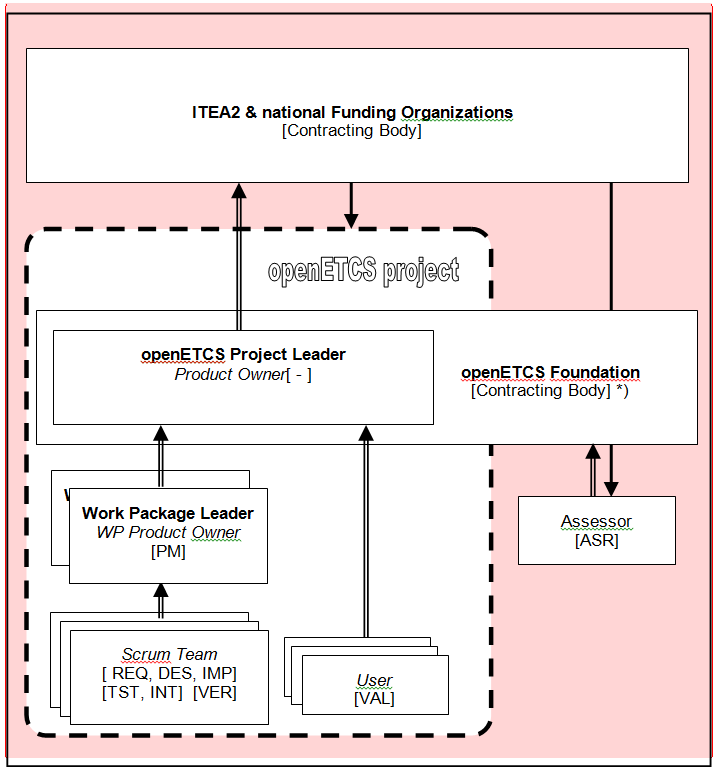
\includegraphics[width=\textwidth]{./figures/organization.PNG}
%\caption{???? Organization ????}
%\end{figure}


\subsection{Committers assignment and responsibilities}
\textit{Proposed  Content: Introduce the concept of Committers as the way to guarantee the required competences are available within the context of the large project, with many organisations involved in the context of a EU project and with an open source environment.  Introduce the concept of Contributors also and the difference between them. Refer to the document where the process to become a Committer and/or contributor is detailed.} \todo[color=yellow!20, inline]{JW: To cover all open source roles also the user have to be introduced.}

\todo[color=yellow!20, inline]{JW: Section covers only open source rules. A short decription of the relations to the project structure and CENELEC rules is needed.}

\subsection{Project QA Management}
\textit{Proposed Content: Provide a description of the tasks to be developed by the project  QA organisational structure jointly with the QA tasks to be performed by the team to guarantee project procedures/{\dots} are met. This means to detail the overall QA strategy.}

\section{Life Cycle}

\todo[color=yellow!20, inline]{JW: A short (two sentences) introduction how these two life cycles are related.}

\subsection{Project Life Cycle }

\todo[color=yellow!20, inline]{JW: A short text before refering to the document (naming of WPs and the overall concept).}
\textit{Proposed Content: Refer to a separate document (PMP and Full Project Proposal)  that describes the WP structure, refer to  the Iterative process; relation between WPs and Results; WP/Project Backlog creation and maintenance and Scrum implementation.}

%\begin{figure}
%\center
%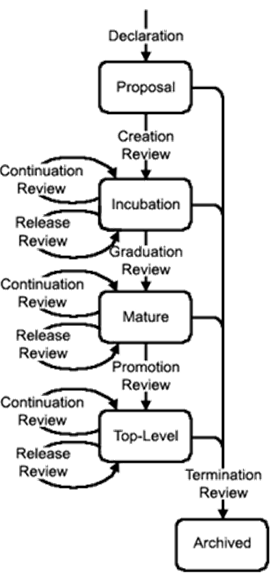
\includegraphics[width=.35\textwidth]{./figures/lifecycle.PNG}
%\caption{???? Lifecycle ????}
%\end{figure}

\subsection{Product Life Cycle }

\todo[color=yellow!20, inline]{JW: Not to long, just short introduction, please.}
\textit{Proposed Content: Refer to a separate document that describes the life cycle. Consider EN50126 and EN50129 Requirements, include Deployment and Maintenance, include activities to "adapt" the generic/abstract software to a concrete implementation.
In this chapter, if applicable, include justification to "potential deviations" to CENELEC standards.}

\subsubsection{Life Cycle of the OpenETCS Software}
\textit{Proposed Content: Prepare a separate document with a complete description of phases of the the SW development life-cycle, including V\&V, QA and Safety processes. This description shall contain the activities to be performed by each role.
In the preparation of this document, contribution of the different WPs is necessary (i.e. WP2 for the Design and development phase and WP4 for the V\&V activities).
In this chapter, if applicable, include justification to "potential deviations" to standard (EN50128) standards.}

\todo[color=yellow!20, inline]{JW: Reference to D 2.3.}

\subsubsection{Life Cycle of the OpenETCS Tools chain}
\textit{Proposed Content: See 3.2.1}

\todo[color=yellow!20, inline]{JW: Reference to the respective documents of WP 7.}

\subsection{QA Management }
\textit{Proposed Content: Refer to the procedures to implement the QA activities identified within the above mentioned development life-cycle. }

\section{Roles}
\subsection{OpenETCS Roles}

\todo[color=yellow!20, inline]{JW: Introduction needed that relates the openETCS project structure based on the open source principles to the needed CENELEC roles. For the specific competencies and the listing the reference can be made to the Annex.}

\textit{Proposed Content: Refer to Annex with the Role/Competence Matrix at project level.
Besides, in this chapter,  outline or refer to the procedure that will be used to maintain this matrix up to date; identify (refer and/or outline) the measures and/or mechanisms in place to record the competencies of the personnel assigned to the different roles (i.e. each company has to maintain training records) and measures and/or mechanisms to identify and fill gaps (i.e.maintain a project specific incorporation programme; maintain a training programme)}

\subsection{Roles within the Development process of the openETCS Software}
\textit{Proposed Content: Refer to Annex with the Role/Competence Matrix of the OpenETCS software. 
Besides in this chapter, outline key specific competences demanded by the ETCS software development to the different roles.}

\subsection{Roles within the Development process of the openETCS Tools Chain}
\textit{Proposed Content: See Chapter 4.2}

\subsection{QA Activities}

\textit{Proposed Content: Describe the measures applied to monitor/verify people assigned to the different roles meet the requirements imposed by the role and have an active/qualified participation to the project (i.e. committers: assess effective contribution activities; gap analysis;{\dots}).}

\section{Methods, measures and tools for quality assurance (product + open ETCS software + Tools chain) + Justification of chosen Tools and Methods}

\todo[color=yellow!20, inline]{JW: The Annex does/can not provide the needed information. Teh references have to be made to the WP 2 and WP3 deliverables, which actually provide these information in depth}

\textit{Proposed Content: Refer to Annex where for each phase in the development life-cycle identify methods and tools as well as justification for selection}

\todo[color=yellow!20, inline]{JW: There should be again sections for the openETCS modell, software (are the product) and Tools chain.}

\subsection{QA Activities}
\textit{Proposed Content: Describe the measures to monitor the appropriate implementation of the selected methods and tools.}

\todo[color=yellow!20, inline]{JW: This is a broad topic, the main issues will be covered by the verification, validation and safety plan. This aspect should introduce the general principals and tools and then reference those documents.}

\section{Documentation}

\subsection{Documentation Structure within the development process of the openETCS Software}
\textit{Proposed Content: Prepare a separate document with a complete description of labelling; definitions and acronyms; control information to include in each document; documents QA criteria; documentation matrix}

\subsection{Documentation Structure within the development process of the openETCS Tools chain}
\textit{Proposed Content: See Chapter 6.1}

\subsection{QA Activities}
\textit{Proposed Content: Describe the methods to review the documentation structure}

\todo[color=yellow!20, inline]{JW: For me this should not be the review of the dcumentation structure, but the documentation quality control activities. These are looked at in detail over the next to chapters, therefore this should be a genereal overview.}

\section{Documentation Control}
\textit{Proposed Content: Refer to Review Process Document where the function develop by authors, reviewers is provider}
\todo[color=yellow!20, inline]{JW: This sentence is hard to understand. From my point of view the three section make no sence sice there should be the same process for all kinds of documents. This section should name the main control activities (review, approval, dissermination, archiving) and the main tools used for this. Then it should refer do the respecitive documents (like the great review process).}

\subsection{Documentation Control within the Development process of the openETCS Sotware}
\textit{Proposed Content: Refer to the list of active documents of the openETCS software}

\subsection{Documentation Control within the Development process of the openETCS Tools chain}
\textit{Proposed Content: Refer to the list of active documents of the openETCS tools chain}

\subsection{QA Activities}
\textit{Proposed Content: Describe the methods to monitor both the control and process}

\section{Tracking and tracing of deviation}


\subsection{Traceability (openETCS software + Tools chain)}
\textit{Proposed Content: Provide a description of traceability requirements, as well as how the traceability will be achieved, implement, maintained and verified. At this stage, exceptions if they exist should be justified.}

\subsection{Configuration Management}
\textit{Proposed Content: Refer to SCMP (System Configuration Management Plan). Overview table with the summary of main features of SCMP.}

\todo[color=yellow!20, inline]{JW: SCMP has to be writen. This mainly includes an explanation of the proper github working processes.}

\textit{Describe the QA activities}

\subsection{Fault Management}
\textit{Proposed Content: Refer to Incident Management Process. Overview table with the summary of main features of the procedure}

\todo[color=yellow!20, inline]{JW: What shall be the be the focus of the "Incident Management", since deal with safety development and Vand V activities, the word incident is mainly used in a safety sence. Here specifically procedures how to handle software bugs and faulty behavior discovered during the V and V process has to be discribed.}

\textit{Describe the QA activities}

\subsection{Grievance Handling}
\textit{Proposed Content: Refer to the specific procedure. }

\textit{Describe the QA activities}

\subsection{Modification and change control }
\textit{Proposed Content: Refer to external procedure; Overview table with the summary of main features of the procedure.}

\todo[color=yellow!20, inline]{JW: What is meant with "external procedures"? This topic is closely related to the document related responsabilities and the github use. Therefore it is very close to the Configuration Management, which maybe makes it hard to seperate these topics.}

\textit{describe the QA activities to be developed.}

\section{Supplier Control}
\textit{Proposed Content: Requirements to external suppliers and how they will be verified}

\todo[color=yellow!20, inline]{JW: What are the suppliers in OpenETCs and what activities are needed here?}

\textit{describe the QA activities to be developed.}

\todo[color=yellow!20, inline]{JW: Im mising sections for the Quality Assurance during the product maintenance and the deploymant of the software and the tool chain.}

\section{ANNEXES}

\subsection{ANNEX A -Role Matrix at project level-}

\begin{description}
\item[Role] Project role
\item[SCRUM] if applicable scrum role
\item[Functions] Responsibilities of the role
\item[Competences Profiles Required] identifier of the competence profile described in the competence matrix
\end{description}

\begin{flushleft}
\tablefirsthead{}
\tablehead{}
\tabletail{}
\tablelasttail{}
\begin{supertabular}{|m{2cm}|m{2cm}|m{9cm}|m{2cm}|}
\hline
\rowcolor{myblue}
Role &
SCRUM &
Functions &
Competence Profiles Required\\\hline
Users &
- &

\begin{itemize}
\item create a viable ecosystem around an openETCS project,
\item encourage additional open source and commercial organizations to participate
\item {\dots}
\end{itemize}
&CPR01, CPR03\\\hline
Adopters &
- &
\begin{itemize}
\item Reuse of the frameworks (within the companies that are contributing to the project and outside of the project),
\item Reuse of the tools (within the companies that are contributing to the project and outside of the project,
\item {\dots}
\end{itemize}

&
CPR03 and CPR04\\\hline

Project Leader &
Product owner &
Text3 &
CPRXX\\\hline
Project Assistant &
OpenETCS Scrum master &
Text3 &
CPRXX\\\hline
Project Contributor &
OpenETCS Scrum team & %\todo[color=blue!40]{JW: This are more external or short term contributers, which do not belong to the team.} &
Text3 &
CPRXX\\\hline
Project Committer &
- &
%\todo[color=blue!40]{JW: This should be the scrum team.} &
Text3 &
CPRXX\\\hline
WP1 Leader &
WP1 product owner &
Text3
&
CPRXX\\\hline
WP1 Assistant &
WP1 Scrum master &
Text3 &
CPRXX\\\hline
WP1 Contributor &
WP1 Scrum team &
Text3 &
CPRXX\\\hline
WP1 Committer &
- &
Text3 &
CPRXX\\\hline
WP2 Leader &
WP2 product owner &

Text3 &
CPRXX\\\hline
WP3 Assistant &
WP3 Scrum master &
Text3 &
CPRXX\\\hline
WP3 Contributor &
WP3 Scrum team  &
Text3 &
CPRXX\\\hline
WP3 Committer &
- &
Text3 &
CPRXX\\\hline
WP4 Leader &
WP4 product owner &
Text3 &
CPRXX\\\hline
WP4 Assistant &
WP4 Scrum master &
Text3 &
CPRXX\\\hline
WP4 Contributor &
WP4 Scrum team  &
Text3 &
CPRXX\\\hline
WP4 Committer &
- &
Text3 &
CPRXX\\\hline
WP5 Leader &
WP5 product owner &
Text3 &
CPRXX\\\hline
WP5 Assistant &
WP5 Scrum master &
Text3 &
CPRXX\\\hline
WP5 Contributor &
WP5 Scrum team  &
Text3 &
CPRXX\\\hline
WP5 Committer &
- &
Text3 &
CPRXX\\\hline
WP6 Leader &
WP6 product owner &
Text3 &
CPRXX\\\hline
WP6 Assistant &
WP6 Scrum master &
Text3 &
CPRXX\\\hline
WP6 Contributor &
WP6 Scrum team  &
Text3 &
CPRXX\\\hline
WP6 Committer &
- &
Text3 &
CPRXX\\\hline
WP7 Leader &
WP7 product owner &
Text3 &
CPRXX\\\hline
WP7 Assistant &
WP7 Scrum master &
Text3 &
CPRXX\\\hline
WP7 Contributor &
WP7 Scrum team  &
Text3 &
CPRXX\\\hline
WP7 Committer &
- &
Text3 &
CPRXX\\\hline
Configuration manager &
- &
Text3 &
CPRXX\\\hline

\end{supertabular}
\end{flushleft}

\todo[color=yellow!40, inline]{JW: "Project Contributor/OpenETCS Scrum team" row --> This are more external or short term contributers, which do not belong to the team.}

\todo[color=yellow!40, inline]{JW: "Project Committer" row --> This should be the scrum team.}

\subsection{ANNEX B -Competence Matrix at project level-}

\begin{description}
\item[Profile Identifier] unique identifier
\item[Competence Description] description of the necessary competences for each profile
\end{description}

\begin{flushleft}
\tablefirsthead{}
\tablehead{}
\tabletail{}
\tablelasttail{}
\begin{supertabular}{|m{3cm}|m{12cm}|}
\hline
\rowcolor{myblue}
Profile identifier&
Competences\\\hline
CPR01 &
Infrastructure (track and signalling) management companies/organisations\\\hline
CPR02 &
\begin{itemize}
\item experience with requirements management process
\item experience with requirements management tools
\item knowledges, experience and deep understanding with subset 026
\item experience in railways sector
\item {\dots}
\end{itemize}\\\hline
CPR03 &
Systems/Subsystems designers and manufacturers\\\hline
CPR04 &
Companies/Organisations that provide solutions/services to rail industry\\\hline
CPR05 &
\begin{itemize}
\item needs to be able to explain the needs and requirements to the developer and must be able to give answers to their questions about details. This does not mean that they need to know everything but a good WP leader knows who knows
\item needs to be able to make decisions on the spot if this is necessary. And a WP leader needs to take responsibility for these decisions,
\item must look at the whole picture and all stakeholders and be able to know which brings the most business value to the product
\item prepared to be involved in conflicts. The biggest challenges in this role just come from the fact that the many different interest and stakeholders are concentrated into a single role
\item {\dots}
\end{itemize}\\\hline
CPR06 &
Text6\\\hline
CPR07 &
Text6\\\hline
CPR08 &
Text6\\\hline
\end{supertabular}
\end{flushleft}

\subsection{ANNEX C -Role Matrix of the OpenETCS software-}
\begin{flushleft}
\tablefirsthead{}
\tablehead{}
\tabletail{}
\tablelasttail{}
\begin{supertabular}{|m{2cm}|m{2cm}|m{9cm}|m{2cm}|}
\hline
\rowcolor{myblue}
CENELEC Roles &
SCRUM &
Functions &
Competence Profiles Required\\\hline
Project Leader &
Product owner &
Text3 &
CPRXX\\\hline
Project Assistant &
Scrum master &
Text3 &
CPRXX\\\hline
Requirement manager &
Scrum team &
\begin{itemize}
\item see cenelec annex
\item {\dots}
\end{itemize}
&
CPRXX\\\hline
Designer &
Scrum team &
Text3 &
CPRXX\\\hline
Implementer &
Scrum team &
Text3 &
CPRXX\\\hline
Tester &
Scrum team &
Text3 &
CPRXX\\\hline
Integrator &
Scrum team &
Text3 &
CPRXX\\\hline
Verifier &
Scrum team &
\begin{itemize}
\item see cenelec annex
\item {\dots}
\end{itemize}
&
CPR09\\\hline
Validator &
Scrum team &
Text3 &
CPRXX\\\hline
Assesor &
Scrum team &
Text3 &
CPRXX\\\hline
\end{supertabular}
\end{flushleft}

\subsection{ANNEX D -Competence Matrix of the OpenETCS software-}

\begin{flushleft}
\tablefirsthead{}
\tablehead{}
\tabletail{}
\tablelasttail{}
\begin{supertabular}{|m{3cm}|m{12cm}|}
\hline
\rowcolor{myblue}
Profile identifier&
Competences\\\hline
CPR09 &
\begin{itemize}
\item must be able to deduce the verification types from the specifications
\item must be competent in various verification methodologies and able to identify the most appropriate method or combination of methods to the context 
\item see cenelec annex
\item {\dots}
\end{itemize}
\\\hline
CPRXX &
Text6\\\hline
CPRXX &
\begin{itemize}
\item see cenelec annex
\item {\dots}
\end{itemize}
\\\hline
CPRXX &
Text6\\\hline
CPRXX &
Text6\\\hline
CPRXX &
Text6\\\hline
CPRXX &
Text6\\\hline
CPRXX &
Text6\\\hline
CPRXX &
Text6\\\hline
CPRXX &
Text6\\\hline
\end{supertabular}
\end{flushleft}

\subsection{ANNEX E -Role Matrix of the OpenETCS Tools chain-}
\begin{flushleft}
\tablefirsthead{}
\tablehead{}
\tabletail{}
\tablelasttail{}
\begin{supertabular}{|m{2cm}|m{2cm}|m{9cm}|m{2cm}|}
\hline
\rowcolor{myblue}
CENELEC Roles &
SCRUM &
Functions &
Competence Profiles Required\\\hline
Project Leader &
Product owner &
Text3 &
CPRXX\\\hline
Project Assistant &
Scrum master &
Text3 &
CPRXX\\\hline
Requirement manager &
Scrum team &
\begin{itemize}
\item see cenelec annex
\item {\dots}
\end{itemize}
&
CPRXX\\\hline
Designer &
Scrum team &
Text3 &
CPRXX\\\hline
Implementer &
Scrum team &
Text3 &
CPRXX\\\hline
Tester &
Scrum team &
Text3 &
CPRXX\\\hline
Integrator &
Scrum team &
Text3 &
CPRXX\\\hline
Verifier &
Scrum team &
Text3 &
CPRXX\\\hline
Validator &
Scrum team &
\begin{itemize}
\item see cenelec annex
\item {\dots}
\end{itemize}
&
CPR09 and CPR12\\\hline
Assesor &
Scrum team &
Text3 &
CPRXX\\\hline
\end{supertabular}
\end{flushleft}

\subsection{ANNEX F -Competence Matrix of the OpenETCS Tools chain-}

\begin{flushleft}
\tablefirsthead{}
\tablehead{}
\tabletail{}
\tablelasttail{}
\begin{supertabular}{|m{3cm}|m{12cm}|}
\hline
\rowcolor{myblue}
Profile identifier&
Competences\\\hline
CPRXX &
Text6\\\hline
CPRXX &
Text6\\\hline
CPRXX &
Text6\\\hline
CPRXX &
Text6\\\hline
CPRXX &
Text6\\\hline
CPRXX &
Text6\\\hline
CPRXX &
Text6\\\hline
CPRXX &
Text6\\\hline
CPR12 &
\begin{itemize}
\item model knowledges
\item {\dots}
\end{itemize}\\\hline
CPRXX &
Text6\\\hline
\end{supertabular}
\end{flushleft}

\subsection{ANNEX G -Methods and tools/Justification for selection-}

\begin{flushleft}
\begin{supertabular}{|m{6cm}|m{2cm}|m{7cm}|}
\hline
\rowcolor{myblue}
\multicolumn{3}{|c|}{Software Design and Implementation} \\\hline
\rowcolor{lightgray}
Method/Technique &
SIL 4 &
Justification\\\hline
Modular Approach &
M &
Text6\\\hline
Components &
HR &
Text6\\\hline
Design and Coding Standards &
M &
Text6\\\hline
Strongly Typed Programming
Language &
HR &
Text6\\\hline
Formal Methods &
HR &
Text6\\\hline
Modeling&
HR &
Text6\\\hline
\end{supertabular}
\end{flushleft}

\begin{flushleft}
\tablefirsthead{}
\tablehead{}
\tabletail{}
\tablelasttail{}
\begin{supertabular}{|m{8cm}|m{7cm}|}
\hline
\rowcolor{myblue}
Quality mechanisms for Safe deployment &
Technique \& Approach\\\hline
Software Self-identification Mechanisms

(9.1.4.11) &
~
\\\hline
Error detection and/or avoidance mechanisms during deployment process (store, transfer, transmission and/or duplication of code operations)

(9.1.4.20) &
~
\\\hline
Automatic detection and safe management of incompatible components/versions

(9.1.4.8, 9.1.4.9) &
~
\\\hline
Provision of appropriate and accurate diagnostic information &
~
\\\hline
Safe Roll back capabilities  &
~
\\\hline
\end{supertabular}
\end{flushleft}

\begin{flushleft}
\tablefirsthead{}
\tablehead{}
\tabletail{}
\tablelasttail{}
\begin{supertabular}{|m{8cm}|m{7cm}|}
\hline
\rowcolor{myblue}
Quality mechanisms for Maintainability &
Technique \& Approach\\\hline
Coding Standards &
~
\\\hline
Impact Assessment &
Before each implementation\\\hline
Data register and analysis &
Creation and maintenance of a project history register\\\hline
Design method selection mechanisms to facility the maintainability (7.3.4.28) &
~
\\\hline
Attenuation actions mechanisms (9.2.4.20) &
~
\\\hline
Mechanisms for evaluating the appropriateness of the methods, tools and techniques used in the modification/maintainability (part of 9.2.4.2 and CENELEC 126 phase 13) &
~
\\\hline
SW description mechanisms (7.1.1.1) &
~
\\\hline
Control mechanisms to guarantee the corrective actions adoption (6.6.4.1) &
~
\\\hline
Provision of appropriate and accurate modification management system (6.6.4.1) and configuration management system (6.5.4.12) &
~
\\\hline
\end{supertabular}
\end{flushleft}

\nocite{EN50126,EN50128,EN50129,EN61508,200857EC,201118EU,201288EU}
\nocite{pichler2010,monin2008,schwaber2008,subset026,subset036,subset076,fpp}

\bibliography{QA_literature}
\bibliographystyle{plain}

\end{document}
